\documentclass[11pt]{article}\usepackage[]{graphicx}\usepackage[]{color}
% maxwidth is the original width if it is less than linewidth
% otherwise use linewidth (to make sure the graphics do not exceed the margin)
\makeatletter
\def\maxwidth{ %
  \ifdim\Gin@nat@width>\linewidth
    \linewidth
  \else
    \Gin@nat@width
  \fi
}
\makeatother

\definecolor{fgcolor}{rgb}{0.345, 0.345, 0.345}
\newcommand{\hlnum}[1]{\textcolor[rgb]{0.686,0.059,0.569}{#1}}%
\newcommand{\hlstr}[1]{\textcolor[rgb]{0.192,0.494,0.8}{#1}}%
\newcommand{\hlcom}[1]{\textcolor[rgb]{0.678,0.584,0.686}{\textit{#1}}}%
\newcommand{\hlopt}[1]{\textcolor[rgb]{0,0,0}{#1}}%
\newcommand{\hlstd}[1]{\textcolor[rgb]{0.345,0.345,0.345}{#1}}%
\newcommand{\hlkwa}[1]{\textcolor[rgb]{0.161,0.373,0.58}{\textbf{#1}}}%
\newcommand{\hlkwb}[1]{\textcolor[rgb]{0.69,0.353,0.396}{#1}}%
\newcommand{\hlkwc}[1]{\textcolor[rgb]{0.333,0.667,0.333}{#1}}%
\newcommand{\hlkwd}[1]{\textcolor[rgb]{0.737,0.353,0.396}{\textbf{#1}}}%
\let\hlipl\hlkwb

\usepackage{framed}
\makeatletter
\newenvironment{kframe}{%
 \def\at@end@of@kframe{}%
 \ifinner\ifhmode%
  \def\at@end@of@kframe{\end{minipage}}%
  \begin{minipage}{\columnwidth}%
 \fi\fi%
 \def\FrameCommand##1{\hskip\@totalleftmargin \hskip-\fboxsep
 \colorbox{shadecolor}{##1}\hskip-\fboxsep
     % There is no \\@totalrightmargin, so:
     \hskip-\linewidth \hskip-\@totalleftmargin \hskip\columnwidth}%
 \MakeFramed {\advance\hsize-\width
   \@totalleftmargin\z@ \linewidth\hsize
   \@setminipage}}%
 {\par\unskip\endMakeFramed%
 \at@end@of@kframe}
\makeatother

\definecolor{shadecolor}{rgb}{.97, .97, .97}
\definecolor{messagecolor}{rgb}{0, 0, 0}
\definecolor{warningcolor}{rgb}{1, 0, 1}
\definecolor{errorcolor}{rgb}{1, 0, 0}
\newenvironment{knitrout}{}{} % an empty environment to be redefined in TeX

\usepackage{alltt}
\usepackage[SOLN]{./../RBmisc}
\usepackage{lipsum}

\newgeometry{top=0.9in,left=1in,right=1in,bottom=0.7in}
\hypersetup{colorlinks=true,urlcolor=blue}
\setlength{\captionmargin}{1em}
\renewcommand{\mean}[1]{\overline{#1}}
%\renewcommand{\sd}[1]{\hat\sigma_{#1}}
\renewcommand{\sd}[1]{s_{#1}}

\def\thisHW{Homework 1}
\def\dueDate{Thu 10 Oct 2019 by 1:30pm}

\rheader{IGP 484, \thisHW}{}{}%{Due: \dueDate}
\IfFileExists{upquote.sty}{\usepackage{upquote}}{}
\begin{document}
\SweaveOpts{concordance=TRUE}




\noindent {This homework assignment involves a lot of sketching \&
a fair bit of algebra.  You may opt to either hand it in \textit{on
paper}, or electronically as a PDF.}  
%The due-date is the same either way.  
%If you wish to hand it in on-paper, you may either turn it in
%during class or slip it under my door: 680 N LSD, Rm 14-065.

\noindent{\textbf{All problems are independent unless stated otherwise.}}


\begin{problems}%enumerate}[itemindent=0em,leftmargin=3ex]

\begin{problem}{%
	Consider the following figure from Kouchoukos, NT \&al.
	``Replacement of the aortic root with a pulmonary autograft
	in children and young adults with aortic-valve disease.'' 
	\textit{New England Journal of Medicine} 330(1), 1994. 
	\url{http://www.ncbi.nlm.nih.gov/pubmed/8259138}
	\begin{center}
		\includegraphics[width=0.75\textwidth]{Kouchoukos.png}
	\end{center}
}	
\probit[3]{Name at least three things wrong with this figure.}
\soln{\\Any of the following:
\begin{itemize}
\item 3-D orientation renders it difficult to discern $y$-values;
\item Data overlap disables one from following individual patient data;
\item No label on the $z$ axis;
\item Cannot discern any overarching trends regarding aortic regurgitation;
\item No purpose for use of triangles/pyramids as data points;
\item Thickness of pyramid bases carry no clear meaning;
\item Shading lowers readability;
\item $\dots$.
\end{itemize}}
\probit[2]{Sketch a better version.}
\soln{\\See attached examples on last page\clearpage}
\end{problem}

\comment{  %%%%%%%%%%%% BEGIN CUT %%%%%%%%%%%%%%%%%%
\begin{problem}{%
	Consider the following figure from Cawley, S \&al.
	``Unbiased mapping of transcription factor binding sites
	along human chromosomes 21 and 22 points to widespread
	regulation of noncoding RNAs.''
	\textit{Cell} 116(4):499-509, 2004.
	\url{http://www.ncbi.nlm.nih.gov/pubmed/14980218}
	\begin{center}
		\includegraphics[width=0.85\textwidth]{Cawley.png}
	\end{center}
}
\probit[3]{Name at least two things wrong with this figure.}
\soln{\\Any of the following:
\begin{itemize}
\item Depth from 3-d orientation carries no meaning;
\item 3-d orientation makes it difficult to perceive relative quantities;
\item Use of pie chart makes it difficult to visually discriminate relative amounts (\eg, the purple section looks bigger than the yellow, even though it represents a smaller percentage);
\item May want to split ``Within or 3' flanking to a known gene'' into two groups;
\item $\dots$.
\end{itemize}}
\probit[2]{Sketch a better version.}
\soln{\\See attached examples on following page\clearpage}
\end{problem}

\probsing[4]{%
	Consider the following figure from Hummer, Li, \& Hassel.
	``Role for p53 in gene induction by double-stranded RNA.''
 	\textit{J Virol} 75, 2001.
	\url{http://www.ncbi.nlm.nih.gov/pubmed/11462054}

	\includegraphics[width=0.97\textwidth]{HummerWide.png}\\
	What problems can you identify with this figure?
}


\begin{problem}{%
	Consider the following figure from Kim, Chung, \& Shin.
	``Higher levels of serum triglyceride and dietary carbohydrate
	intake are associated with smaller LDL particle size in
	healthy Korean women.'' 
	\textit{Nutr Res Pract.} 6(2), 2012.
	\url{http://www.ncbi.nlm.nih.gov/pubmed/22586500}
	\begin{center}
		\includegraphics[width=0.7\textwidth]{Kim.png}
	\end{center} 
}
\probit[2]{Is this figure a histogram?  Justify your answer.}
\probit[4]{Describe in words what this figure shows and give your interpretation of it.}
\probit[4]{How would you improve this figure?  Sketch an improved version.}
\end{problem}
}  %%%%%%%%%%%%%% END CUT %%%%%%%%%%%%%

\begin{problem}{%
Consider the following set of measurements of some variable $x$:
%\vspace{-1ex}
\begin{center}
% latex table generated in R 4.1.1 by xtable 1.8-4 package
% Sun Sep 19 09:11:24 2021
\begin{tabular}{rrrrrrrrrr}
   52 &  16 & 180 &   1 & 199 &   8 &   3 &  23 & 156 &  63 \\ 
  808 &  25 &   5 & 554 &  85 &   1 &  64 &  52 &   7 & 192 \\ 
  \end{tabular}

\end{center}
%\vspace{-4ex}
}
\probit[3]{Using a handheld calculator, compute:
	%or computer software of your choosing%
	%\footnote{If you want, you can put these values into R with:\\
	%\texttt{paste0("x <- ",paste(deparse(x),collapse=""))}
	%},
	\soln{\\Be mindful of significant digits -- your mean, median, and SD should not be reported to greater precision than your data was! (TA's: mark sig digs, but do not deduct points.)}
	\begin{itemize}
	\item The mean of $x$\soln{=125}.
	\item The median of $x$\soln{=52}.
	%\item The geometric mean of $x$\soln{=round(prod(x)^(1/length(x)))}.
	\item The sample standard deviation of $x$\soln{=206}.
	\end{itemize}
\vspace{1ex}
}
\probit[6]{Sketch:
		\begin{itemize}
		\item  a rough histogram of $x$
\soln{(0 pts if axes are unlabeled or not approximately numbered)
\vspace{-2em}
\begin{knitrout}
\definecolor{shadecolor}{rgb}{0.969, 0.969, 0.969}\color{fgcolor}

{\centering 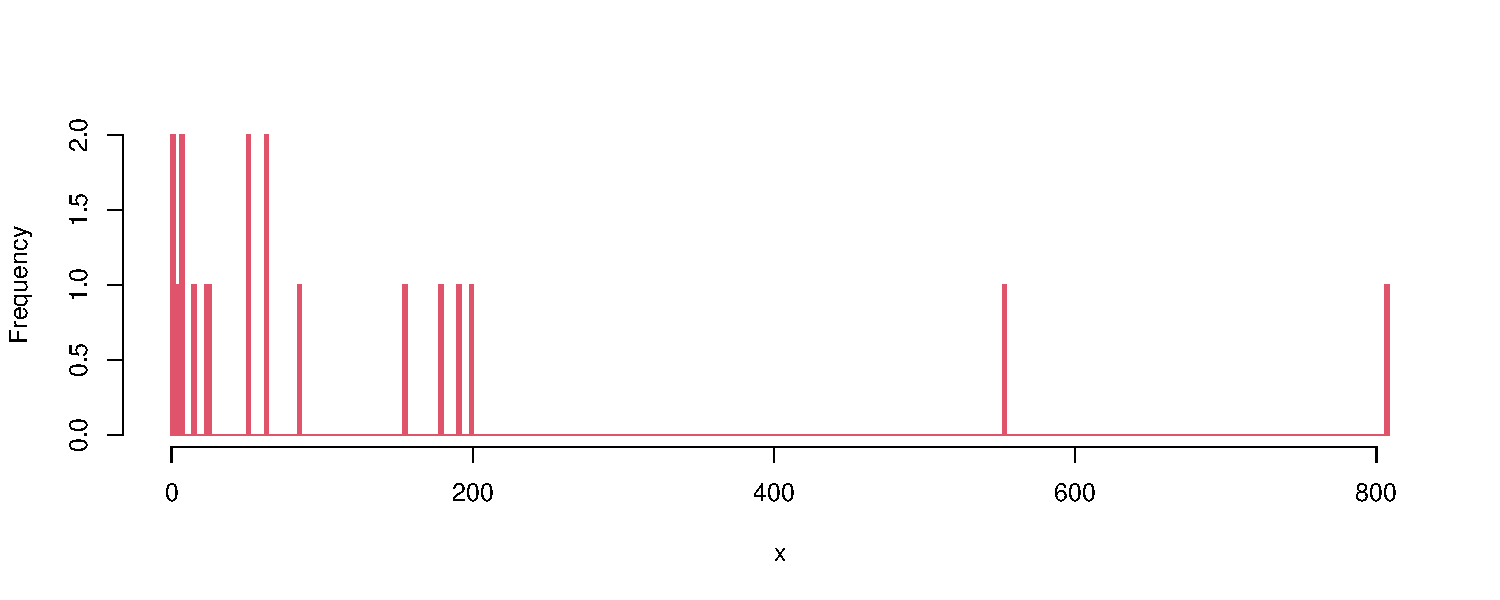
\includegraphics[width=.9\linewidth]{figure/histx-1} 

}


\end{knitrout}
\vspace{-1em}
}
		\item a rough boxplot of $x$ \soln{(Vertical is ok too!  0 pts if axis is not approximately numbered)
\vspace{-2em}
\begin{knitrout}
\definecolor{shadecolor}{rgb}{0.969, 0.969, 0.969}\color{fgcolor}

{\centering 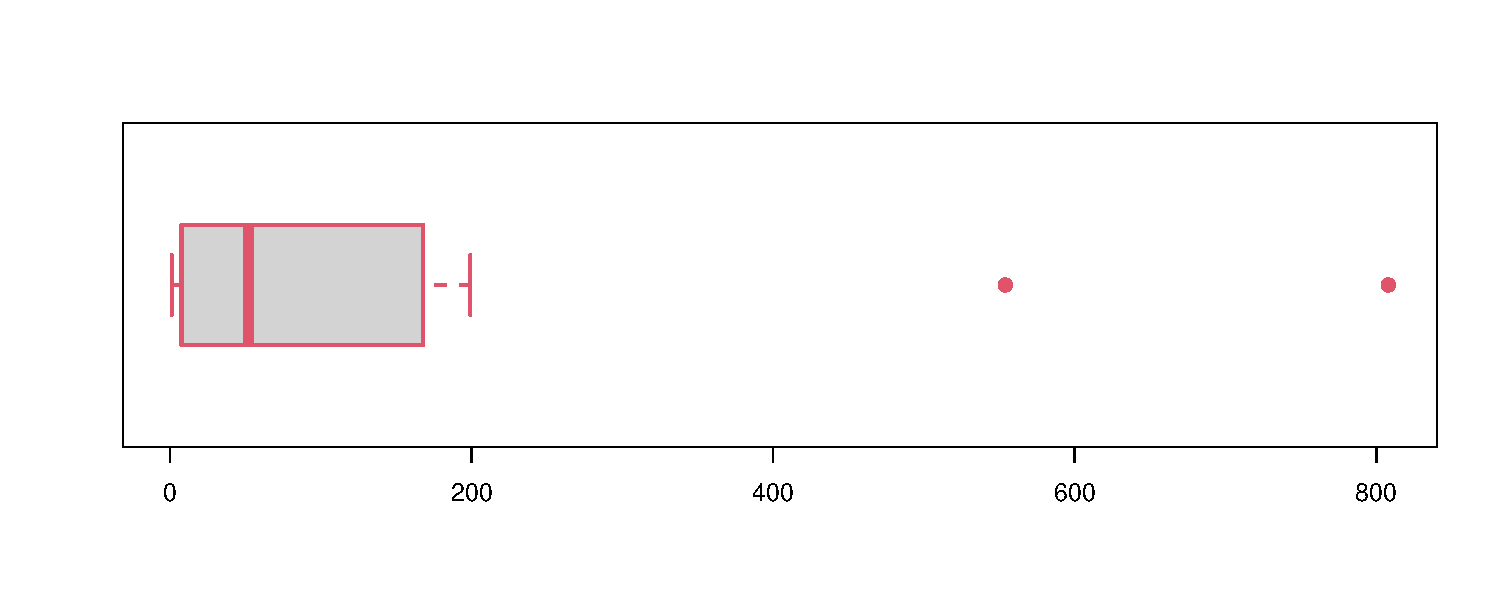
\includegraphics[width=.9\linewidth]{figure/boxpx-1} 

}


\end{knitrout}
\vspace{-2em}}
\end{itemize}
and describe the shape of the distribution in words.
\soln{\\The distribution of the data is heavily skewed to the right.}
\vspace{1ex}
}
%\ifthenelse{\boolean{wSoln}}{}{\clearpage}

%	\probit[8]{Compute:% 
%\begin{itemize}
%	\item the mean and sample SD of $2x$.\soln{ round(c(mean=mean(2*x),sd=sd(2*x)))}
%	\item the mean and sample SD of $x+10$.\soln{ round(c(mean=mean(x+10),sd=sd(x+10)))}
%	\item the mean and sample SD of $2x+10$.\soln{ round(c(mean=mean(2*x+10),sd=sd(2*x+10)))}
%	\item the mean and sample SD of $2(x+10)$.\soln{ round(c(mean=mean(2*(x+10)),sd=sd(2*(x+10))))}
%	\end{itemize}
%}
	\probit[3]{Suppose we added two additional observations to $x$, both of which were exactly equal to
the mean of $x$ (as obtained in part (a) above). 
\soln{\\
(TA's: please grade this based on the solution given for (a), even if (a) was wrong.  
Ie, answers that are consistent with (a) are correct; inconsistency w/ (a) is \textit{incorrect}.)

}
	\begin{itemize}
	\item What would the new mean be? \soln{ \framebox{125}}
	\item What would the new median be? \soln{ \framebox{58}}
	\item What would the new sample SD be? \soln{ \framebox{196}\clearpage}
	\end{itemize}
}
\end{problem}

\begin{problem}{%
Recall the definitions of the sample mean and sample standard deviation:
\begin{align*}
\mean{x} = \frac{1}{N} \sum_{i=1}^N x_i \quad ; \qquad%\\
\sd{x} = \sqrt{\frac{1}{N-1} \sum_{i=1}^N (x_i - \mean{x})^2} \quad.
\end{align*}
Suppose $x$ is a \textit{sample of body temperatures in Fahrenheit}
from patients admitted to the ER in the past month. 
Let $y$ be that same set of measurements, but converted to Celsius.
}
\probit[1]{Write down the equation for
obtaining $y$ as a function of $x$.} \soln{
\[y=\frac{5}{9}(x-32)\]
Note that this is a \textit{linear transformation}, \ie, $y$ has the form $mx+b$.}
\probit[3]{If $\mean{x}$ is the mean of the Fahrenheit measurements, what would the mean of the Celsius
measurements $\mean{y}$ be, in terms of $\mean{x}$?  (Ie: derive an equation for $\mean{y}$ as a function $\mean{x}$.) \textbf{Show your work.}}\soln{
\\NB: 0 points if no work is shown, even if the answer is correct.
\begin{align*}
\mean{y} &= \frac{1}{N} \sum_{i=1}^N y_i \\
&= \frac{1}{N} \sum_{i=1}^N \frac{5}{9}(x_i-32) \\
&= \frac{1}{N} \frac{5}{9} \sum_{i=1}^N (x_i-32) \\
&= \frac{1}{N} \frac{5}{9} \left(\sum_{i=1}^N x_i - \sum_{i=1}^N 32\right)\\
&= \frac{1}{N} \frac{5}{9} \left(\sum_{i=1}^N x_i - 32 N \right) \\
&= \frac{5}{9} \left(\frac{1}{N} \sum_{i=1}^N x_i - \frac{1}{N} 32 N \right) \\
&= \frac{5}{9} \left(\mean{x} - 32 \right) \,. 
\end{align*}
That is, the mean of the Celsius--converted values $y$ is the same as taking the mean of the Fahrenheit values $\mean{x}$ and converting it after the fact.  In general, the mean of linearly transformed data is the same as the linear transformation of the mean.  Note, however, that this only holds for linear transformations; other types of transformations do not have this property.  For example, the mean of $x^2$ (\ie, $\mean{x^2}$) is not the same as the $($mean of $x)^2$ (\ie, $\mean{x}^2$).\clearpage}
\probit[3]{If $\sd{x}$ is the sample SD of the Fahrenheit measurements, what would the sample SD 
of the Celsius measurements $\sd{y}$ be, in terms of $\sd{x}$?  (Ie: derive an equation for $\sd{y}$ as a function of $\sd{x}$.) \textbf{Show your work.}} \soln{
\\NB: 0 points if no work is shown, even if the answer is correct.
\begin{align*}
\sd{y} &= \sqrt{\frac{1}{N-1} \sum_{i=1}^N (y_i - \mean{y})^2}\\
&= \sqrt{\frac{1}{N-1} \sum_{i=1}^N \left(\frac{5}{9}(x_i-32) - \frac{5}{9}(\mean{x}-32) \right)^2}\\
&= \sqrt{\frac{1}{N-1} \sum_{i=1}^N \left(\frac{5}{9}(x_i-32-\mean{x}+32)\right)^2}\\
&=\sqrt{\frac{1}{N-1} \sum_{i=1}^N \left(\frac{5}{9}(x_i-\mean{x})\right)^2}\\
&=\sqrt{\frac{1}{N-1} \left(\frac{5}{9}\right)^2  \sum_{i=1}^N (x_i-\mean{x})^2}\\
&=\abs{\frac{5}{9}} \sqrt{\frac{1}{N-1} \sum_{i=1}^N (x_i-\mean{x})^2}\\
&=\abs{\frac{5}{9}} \sd{x} \,.
\end{align*}
Note that the standard deviation of the linearly transformed data is \textit{NOT} the same as a linear transformation of the SD!
}
\end{problem}

\begin{problem}{In this problem, we will consider a few properties of the geometric mean:
\begin{align*}
\mathrm{Geom.Mean}(x) &= \sqrt[N]{\prod_{i=1}^N x_i} \\
&=(x_1 \cdot x_2 \cdot x_3 \cdots x_N)^\frac{1}{N}\, .
\end{align*}
}
\probit[2]{Compute the geometric mean of the sample $x$ given in Problem 2.
\soln{\framebox{34}\\}
How does it compare to the other measures of central tendency you got in 3(a)?}
\soln{\\ It is much lower than the mean of this very skewed distribution.  It is also lower than the median, but much closer to the median than the mean. It seems to be a more reasonable summary of the data than the arithmetic mean, as it is not driven by the high outlying points.}
\probit[2]{Suppose that one of the measurements of a sample is equal to $0$.  What would the geometric mean of the sample be?} \soln{\\ If a single measurement is 0, the geometric mean will always be 0, regardless of what any of the other measurements are.\clearpage}
\probit[2]{Suppose that one of the measurements of a sample is negative.  What can you say about its geometric mean?  (Hint: consider a case with a sample-size of $N=2$, where one sample is negative; then consider $N=3$.)}
\soln{\\ If one or more measurements are negative, the geometric mean will either be unsolvable or invalid.  In the case of a single negative sample, the geometric mean will either be imaginary for an even number of samples (\eg, $N=2$) or will be necessarily negative regardless of all the other values when there are an odd number of samples (\eg, $N=3$).  This argument also applies for greater odd numbers of negative values; in the case of an even number of negative values, the geometric mean would turn out to be positive, even if they are \textit{all} negative!}
\probit[2]{Given your answers to (a--c), under what circumstances would the geometric mean be useful?}
\soln{\\ In (b), we saw that a single 0 renders the geometric mean useless, since it ``overrides'' any other data.  In (c), we saw that having any negative values makes the geometric mean either imaginary (trying to take an even root of a negative product) or invalid (misleadingly signed).  We thus conclude that \textit{the geometric mean is ONLY valid when ALL measurements $>0$ !}  Part (a) shows that it can be a useful summary when these conditions are met and the distribution of the data are significantly skewed and/or feature outliers.  

The geometric mean is closely related to the arithmetic mean of the log of the values.  Specifically, $\log(\mathrm{Geom.Mean}(x))=\mean{\ln(x)}$.  You can prove this with a little algebra---try it!}
%\item \qpts{5} Recall that $\log(a^b)=b \log(a)$ and $\log(a{\cdot}b)=\log(a)+\log(b)$ \soln{=round(exp(mean(log(x))))}
\end{problem} 


\begin{problem}{Suppose a  test is 99\% accurate:
it gives a positive 
result 99\% of the time if the patient is indeed
infected (\ie a 1\% false-negative rate), 
and a negative result 99\% of the time
if the patient is indeed healthy (\ie a 1\%
false-positive rate). 
For convenience, let +/-- 
denote a positive/negative test result, and
let I/$\bar{\mathrm{I}}$ denote 
infected/well, respectively.}

\probit[2]{Using $\Pr(\cdot|\cdot)$ notation, write down the facts
described above.}\soln{$\Pr(+|I)=0.99$, $\Pr(-|\bar{I})=0.99$, 
$\Pr(-|I)=0.01$, $\Pr(+|\bar{I})=0.01$.  NB: giving just the first two
or the 2nd two is sufficient.}

\probit[1]{Suppose I take the test and it comes up positive.  I'd like
to know what that means about the chances that I'm actually infected.
Using $\Pr(\cdot|\cdot)$ notation, write down the quantity I'm
interested in (NB, not the number, just the notation for the conditional
probability that corresponds to this question).}\soln{$\Pr(I|+)$}

\probit[4]{Supposing my test came up positive, what can you tell me
about the chances that I'm actually infected?  Give numbers if you can;
if you can't, state what else you'd need to know. 
[Hint: remember that the probability of a positive result
is the sum of the probabilities of getting a true positive or
of getting a false positive, \ie, 
$\Pr(+)=\Pr(+|I)\ \Pr(I)+\Pr(+|\bar{I})\ \Pr(\bar{I})$,
and that $\Pr(\bar{I})=1-\Pr(I)$.]
\soln{\\Per Bayes thm, 
\begin{align*}
\Pr(I|+)&=\frac{\Pr(+|I)\ \Pr(I)}{\Pr(+)}\\
&=\frac{\Pr(+|I)\ \Pr(I)}{\Pr(+|I)\ \Pr(I)+\Pr(+|\bar{I})\ \Pr(\bar{I})}\\
&=\frac{\Pr(+|I)\ \Pr(I)}{\Pr(+|I)\ \Pr(I)+\Pr(+|\bar{I})\ (1-\Pr(I))}\\
&=\frac{0.99\ \Pr(I)}{0.99\ \Pr(I)+0.01\ (1-\Pr(I))}\, .
\end{align*}
To solve this, we need to know $\Pr(I)$, the probability I'm
infected regardless of the test result.  This is not known.}}


\probit[4]{Suppose we administered the test in a population where the
prevalence of infection (\ie, the baseline probability that a given
person is infected) is  1/1000. That is, $\Pr(I)=0.001$.\begin{itemize}
\item What fraction of all people would have a positive test result?
\soln{$\Pr(+)=\Pr(+|I)\ \Pr(I)+\Pr(+|\bar{I})\ \Pr(\bar{I})=0.01098$}
\item Of those people, what fraction of them would be truly infected?
\soln{$\frac{\Pr(+|I)\ \Pr(I)}{\Pr(+)}=\\0.00099/0.01098=0.09$}
\item What is the probability, then, that a person in this population
with a positive result is truly infected?  (NB: we call this the 
\textit{posterior probability} or the \textit{positive predictive
value}.)\soln{0.09}
\item Should people in this population believe that they're more
likely infected than not
if they get a positive test result? \soln{No; there is only a 9\% 
chance they're infected!}
\item Does this answer surprise you?  Why or why not?
\end{itemize}}

\probit[3]{Suppose now we do the same thing, but in a high-risk
population where the prevalence is 1/3.  How do your answers 
to (d) change? \soln{The PPV goes up to 0.98!  A positive result
is much more reliable here.} Between this result and your
answer to part (d), what kind of recommendations would you make
for administering this screening test? \soln{It probably only
makes sense to administer this test in a high-risk population,
since a positive result would be much more reliable}}

\probit[4]{Suppose we go back to the low-risk group in (d) and 
re-administer the same test to those who tested positive the first
time.  What is the probability that someone who tests positive a
second time (in addition to the first) is truly infected?}
\soln{Of the people who got a $+$ result, 0.09 are infected,
so retesting in that population is like setting $\Pr(I)=0.09$.
Testing them gives a PPV of $0.907$.  Testing positive \textit{twice}
is much more reliable than just testing positive once.}

%\probit[5]{How many times ($N$) would I have to readminister
%this test to the consistently positive people before I
%could say that having $N$ consecutive positive results
%implies a $>50\%$ chance that the patient is truly infected?
%(Note: you can either solve this algebraically or do the 
%computation by hand, incrementing $N$ until the posterior 
%probability is ${>}0.5$.  Show all your work either way.)}

\end{problem}



\end{problems} 
\end{document}
